% !TeX spellcheck = en_US
\documentclass[a4paper,12pt]{report}

\usepackage{color}
\usepackage{float}
\usepackage{babel}
\usepackage{fourier}
\usepackage{amsmath}
%% \usepackage{dirtree} %to show tree view directories.
\usepackage{caption}
\usepackage{nomencl}
\usepackage{verbatim}
\usepackage{fancyhdr}
\usepackage{graphicx}
\usepackage{geometry}
\usepackage{outlines}
\usepackage{enumitem}
\usepackage{fancyvrb}
\usepackage{listings}
\usepackage{makecell}
\usepackage{tabularx} % for custom width table
\usepackage{subcaption}
\usepackage{datenumber}
\usepackage{indentfirst}
\usepackage{lstautogobble}
\usepackage[table]{xcolor}
\usepackage[utf8]{inputenc}
\usepackage[space]{grffile}
\usepackage[final]{pdfpages}
\usepackage[datesep=.,calc,showdow]{datetime2}

%% \usepackage[perpage]{footmisc}
\usepackage[breakable]{tcolorbox}
\tcbuselibrary{breakable, skins}
\usepackage[Bjornstrup]{fncychap}
%Options: Sonny, Lenny, Glenn, Conny, Rejne, Bjarne, Bjornstrup
\usepackage[colorlinks,linkcolor=blue,citecolor=red,urlcolor=blue]{hyperref}

%% \usepackage[style=long,toc,xindy]{glossaries}
%% \usepackage[symbols,nogroupskip,sort=standard]{glossaries-extra}

\usepackage[fontsize={12,18}]{xepersian}

\DTMsetup{useregional}

% -------------- tcolorbox -------------
\tcbset{
	enhanced,
	colback=cyan!5!white,
	boxrule=0.1pt,
	colframe=cyan!75!black,
	fonttitle=\bfseries,
	width=0.9\linewidth
}
% ------------- font setup -------------
% ------------- xepersian --------------
%% \settextfont{Microsoft Sans Serif}
\settextfont{Yas}
\setlatintextfont{Times New Roman}
\setmathdigitfont{Yas}

\defpersianfont\XBT[Scale=1.1]{XB Titre}
\deflatinfont\FS[Scale=16]{Far.Symbol8}
\deflatinfont\TNR[Scale=1]{Times New Roman}

\newcommand*{\CNSLS}{\fontfamily{Consolas}\selectfont}

% --------------   xcolor  -------------
\definecolor{ao}{rgb}			{0.00, 0.50, 0.00}
\definecolor{codeGreen}{rgb}	{0.00, 0.50, 0.50}
\definecolor{lavendergray}{rgb}	{0.87, 0.86, 0.92}
\definecolor{mint}{rgb}			{0.24, 0.71, 0.54}
\definecolor{aliceblue}{rgb}	{0.94, 0.97, 1.00}
\definecolor{commentGreen}{rgb}	{0.13, 0.65, 0.47}
\definecolor{steelBlue}{rgb}	{0.00, 0.00, 0.50}
\definecolor{stringGreen}{rgb}	{0.00, 0.50, 0.00}
\definecolor{rowBlue}{rgb}		{0.48, 0.81, 0.87}

% ---------  page header setup ---------
% --------------  fancyhdr -------------
\pagestyle{fancy}

\cfoot{\thepage}
\rhead{\thepage }
\renewcommand{\headrulewidth}{0.4pt}

%% new commands.
\newcommand{\lrm}[1]{\textcolor{steelBlue}{\lr{\texttt{#1}}}}

%% tabular borders color
\arrayrulecolor{gray}

\renewcommand{\bibname}{مراجع}
% \newglossaryentry{dot-product}{name={dot product},description={aaa}}
% \makeglossaries
\makenomenclature
\renewcommand{\nomname}{فهرست علائم}
\nomenclature{$\bullet$}{bullet}

%% outline settings
% \newcommand{\labelcenumi}{$\bullet$}
% \setlist[itemize]{label = $\bullet$ }

\begin{document}
	\lstset{
		frame=tb,
		basicstyle=\color{steelBlue}\linespread{0.8}\ttfamily,
		columns=fullflexible,
		keepspaces=false,
		tabsize=4,
		autogobble,
		breaklines=true,
		breakatwhitespace=true,
		stringstyle=\color{stringGreen},
		commentstyle=\color{gray},
		keywordstyle=\color{purple},
		language=java,
		aboveskip=3mm,
		belowskip=3mm,
		showstringspaces=false,
		columns=flexible,
		captionpos=b,
		numbers=left,
		numbersep=5pt,
		numberstyle=\color{gray}\linespread{0.8}\ttfamily,
		postbreak=\mbox{\textcolor{blue}{$\hookrightarrow$}\space}
	}

	\renewcommand{\bibname}{مراجع}
	\thispagestyle{empty}


	\begin{center}
		{
			\qquad\textcolor{gray}{\FS 2}
		}
	\end{center}\vspace*{5cm}
	\begin{figure}[h]
		\centering
		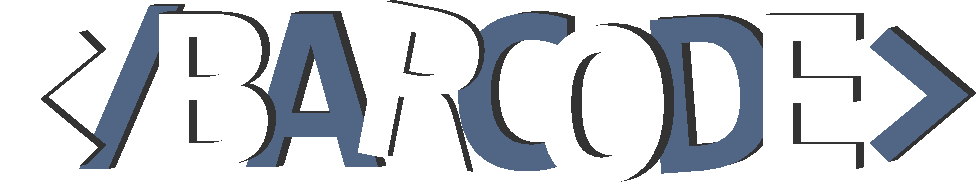
\includegraphics[width=.8\linewidth]{resources/BarcodeLogo.pdf}\\
		\label{barcode-logo}
	\end{figure}
	\title{
		\XBT
		راهنمای تیم بارکد\\
		همراه با کد‌های آماده برای مسابقات
	}
	\author{
		\XBT
		تیم بارکد
		\lr{\XBT (Barcode)}
	}
	\date{
		\XBT\today
	}

	\pagenumbering{roman}
	\maketitle
	\tableofcontents
	\pagenumbering{arabic}

	\chapter*{مقدمه}\label{chap0}
	\addcontentsline{toc}{chapter}{
	مقدمه}

	\chapter{
	کد‌های آماده
	\lr{(Cheat Sheets)}
	}\label{chap1}

	% =============================== c++ section ================================
	\section{\lr{C++}}\label{sec1:chap1}
	\subsection{\lr{Dijkstra}}\label{subsec1:sec1:chap1}
	لینک برگرفته شده از سایت
	\hyperref{https://www.geeksforgeeks.org}{algorithmSite}{geeksforgeeks}{\lr{geeks for geeks}}
	الگوریتم
	\hyperref{https://www.geeksforgeeks.org/dijkstras-shortest-path-algorithm-greedy-algo-7/}{DijkstraAlgorithm}{geeksforgeeks}
	{\lr{Dijkstra’s shortest path algorithm}}.
	\cite{Geeksfor41:online}


	\begin{latin}
		\small
		\begin{lstlisting}[language=C++]
		#include <climits>
		#define V 9

		int minDistance(int dist[], bool sptSet[]) {
			int min = INT_MAX, min_index;
			for (int v = 0; v < V; v++)
			if (sptSet[v] == false && dist[v] <= min)
			min = dist[v], min_index = v;
			return min_index;
		}

		void dijkstra(int graph[V][V], int src) {
			int dist[V];
			bool sptSet[V];
			for (int i = 0; i < V; i++)
			dist[i] = INT_MAX, sptSet[i] = false;
			dist[src] = 0;
			for (int count = 0; count < V - 1; count++) {
				int u = minDistance(dist, sptSet);
				sptSet[u] = true;
				for (int v = 0; v < V; v++)
				if (!sptSet[v] && graph[u][v] && dist[u] != INT_MAX &&
										 dist[u] + graph[u][v] < dist[v])
					dist[v] = dist[u] + graph[u][v];
			}
			printSolution(dist);
		}
		\end{lstlisting}
	\end{latin}

	\subsection{\lr{Segment Tree}}\label{subsec2:sec1:chap1}

	لینک برگرفته شده از سایت
	\hyperref{https://www.geeksforgeeks.org}{algorithmSite}{geeksforgeeks}{\lr{geeks for geeks}}
	الگوریتم
	\hyperref{https://www.geeksforgeeks.org/segment-tree-efficient-implementation/}{Segment tree}{geeksforgeeks}
	{\lr{Dijkstra’s shortest path algorithm}}.
	\cite{Geeksfor41:online}
	\begin{latin}
		\small
		\begin{lstlisting}[language=C++]
		const int N = 100000;
		int n;
		int tree[2 * N];

		void build( int arr[]) {
			for (int i=0; i<n; i++)
				tree[n+i] = arr[i];
			for (int i = n - 1; i > 0; --i)
				tree[i] = tree[i<<1] + tree[i<<1 | 1];
		}

		void updateTreeNode(int p, int value) {
			tree[p+n] = value;
			p = p+n;
			for (int i=p; i > 1; i >>= 1)
				tree[i>>1] = tree[i] + tree[i^1];
		}

		int query(int l, int r) {
			int res = 0;
			for (l += n, r += n; l < r; l >>= 1, r >>= 1) {
				if (l&1)
					res += tree[l++];
				if (r&1)
					res += tree[--r];
			}
			return res;
		}
		\end{lstlisting}
	\end{latin}

	\subsection{\lr{Big Int Multiplication}}\label{subsec4:sec1:chap1}
	\lr{revise needed...}
	\begin{latin}
		\small
		\begin{lstlisting}[language=C++]
		 #include <string>
		 #include <algorithm>

		string multiplication(string str1, string str2)	{
			int len1 = str1.length(), len2 = 0, olen = 0;
			string res(len1 + len2, 0);
			for (int i = 0; i <len2; i++) {
				for (int j = 0; j <len1; j++) {
					res[j + i] += (str1[len1 - j - 1] - 48) * (str2[len2 - i - 1] - 48);
					olen = j + i + 1;
					if (res[j + i] >= 10) {
						res[j + i + 1] += res[j + i] / 10;
						res[j + i] = res[j + i] % 10;
						olen = j + i + 2;
					}
				}
			}
			string reverseOut = reverse(res.begin(),res.end());
			return reverseOut;
		}
		\end{lstlisting}
	\end{latin}

	\subsection{\lr{K-D tree}}\label{subsec5:sec1:chap1}
	لینک برگرفته شده از سایت
	\hyperref{https://www.geeksforgeeks.org}{algorithmSite}{geeksforgeeks}{\lr{geeks for geeks}}
	الگوریتم
	\hyperref{https://www.geeksforgeeks.org/k-dimensional-tree/}{K D-tree}{geeksforgeeks}
	{\lr{kd-tree}}.
	\cite{Geeksfor41:online}
	\begin{latin}
		\small
		\begin{lstlisting}[language=C++]
		 #include<bits/stdc++.h>
		 using namespace std;

		 const int k = 2;

		 struct Node {
		 	int point[k];
		 	Node *left, *right;
		 };

		 struct Node* newNode(int arr[]) {
		 	struct Node* temp = new Node;
		 	for (int i=0; i<k; i++)
		 		temp->point[i] = arr[i];
		 	temp->left = temp->right = NULL;
		 	return temp;
		 }

		 Node *insertRec(Node *root, int point[], unsigned depth) {
		 	if (root == NULL)
		 		return newNode(point);
		 	unsigned cd = depth % k;
		 	if (point[cd] < (root->point[cd]))
		 		root->left = insertRec(root->left, point, depth + 1);
		 	else
		 		root->right = insertRec(root->right, point, depth + 1);
		 	return root;
		 }

		 Node* insert(Node *root, int point[]) {
		 	return insertRec(root, point, 0);
		 }

		 bool arePointsSame(int point1[], int point2[]) {
		 	for (int i = 0; i < k; ++i)
			 	if (point1[i] != point2[i])
			 		return false;
		 	return true;
		 }

		 bool searchRec(Node* root, int point[], unsigned depth) {
		 	if (root == NULL)
		 		return false;
		 	if (arePointsSame(root->point, point))
		 		return true;

		 	unsigned cd = depth % k;
		 	if (point[cd] < root->point[cd])
		 		return searchRec(root->left, point, depth + 1);
		 	return searchRec(root->right, point, depth + 1);
		 }

		 bool search(Node* root, int point[]) {
		 	return searchRec(root, point, 0);
		 }

		 int main() {
		 	struct Node *root = NULL;
		 	int points[][k] = {{3, 6}, {17, 15}, {13, 15}, {6, 12}, {9, 1}, {2, 7}, {10, 19}};

		 	int n = sizeof(points)/sizeof(points[0]);

		 	for (int i=0; i<n; i++)
			 	root = insert(root, points[i]);

		 	int point1[] = {10, 19};
		 	(search(root, point1))? cout << "Found\n": cout << "Not Found\n";

		 	int point2[] = {12, 19};
		 	(search(root, point2))? cout << "Found\n": cout << "Not Found\n";

		 	return 0;
		 }

		\end{lstlisting}
	\end{latin}

	\subsection{\lr{Longest Common Subsequence}}\label{subsec6:sec1:chap1}
	لینک برگرفته شده از سایت
	\hyperref{https://www.geeksforgeeks.org}{algorithmSite}{geeksforgeeks}{\lr{geeks for geeks}}
	الگوریتم
	\hyperref{https://www.geeksforgeeks.org/k-dimensional-tree/}{LCS}{geeksforgeeks}
	{\lr{Longest Common Subsequence}}.
	\cite{Geeksfor41:online}
	\begin{latin}
		\small
		\begin{lstlisting}[language=C++]
		 #include<bits/stdc++.h>
		 using namespace std;
		 int max(int a, int b);
		 int lcs( char *X, char *Y, int m, int n ) {
		 	int L[m + 1][n + 1];
		 	int i, j;
		 	for (i = 0; i <= m; i++) {
		 		for (j = 0; j <= n; j++) {
		 			if (i == 0 || j == 0)
		 				L[i][j] = 0;
		 			else if (X[i - 1] == Y[j - 1])
		 				L[i][j] = L[i - 1][j - 1] + 1;
		 			else
		 				L[i][j] = max(L[i - 1][j], L[i][j - 1]);
		 		}
		 	}
		 	return L[m][n];
		 }

		 int max(int a, int b) {
		 	return (a > b)? a : b;
		 }

		 int main() {
		 	char X[] = "AGGTAB";
		 	char Y[] = "GXTXAYB";
		 	int m = strlen(X);
		 	int n = strlen(Y);
		 	cout << "Length of LCS is "	<< lcs( X, Y, m, n );
		 	return 0;
		 }
		\end{lstlisting}
	\end{latin}

	\subsection{\lr{Longest Common Subsequence}}\label{subsec6:sec1:chap1}
	لینک برگرفته شده از سایت
	\hyperref{https://www.geeksforgeeks.org}{algorithmSite}{geeksforgeeks}{\lr{geeks for geeks}}
	الگوریتم
	\hyperref{https://www.geeksforgeeks.org/k-dimensional-tree/}{LCS}{geeksforgeeks}
	{\lr{Longest Common Subsequence}}.
	\cite{Geeksfor41:online}
	\begin{latin}
		\small
		\begin{lstlisting}[language=C++]
		 #include<bits/stdc++.h>
		 using namespace std;
		 int max(int a, int b);
		 int lcs( char *X, char *Y, int m, int n ) {
		 	int L[m + 1][n + 1];
		 	int i, j;
		 	for (i = 0; i <= m; i++) {
		 		for (j = 0; j <= n; j++) {
		 			if (i == 0 || j == 0)
		 				L[i][j] = 0;
		 			else if (X[i - 1] == Y[j - 1])
		 				L[i][j] = L[i - 1][j - 1] + 1;
		 			else
		 				L[i][j] = max(L[i - 1][j], L[i][j - 1]);
		 		}
		 	}
		 	return L[m][n];
		 }

		 int max(int a, int b) {
		 	return (a > b)? a : b;
		 }

		 int main() {
		 	char X[] = "AGGTAB";
		 	char Y[] = "GXTXAYB";
		 	int m = strlen(X);
		 	int n = strlen(Y);
		 	cout << "Length of LCS is "	<< lcs( X, Y, m, n );
		 	return 0;
		 }
		\end{lstlisting}
	\end{latin}

	\subsection{\lr{algorithm name}}\label{subsec0:sec1:chap1}
	%\subsubsection{}\label{subsubsec1:subsec1:sec1:chap1}


	% ============================ python section ================================
	\section{\lr{Python}}\label{sec2:chap1}
	\subsection{\lr{algorithm name}}\label{subsec1:sec2:chap1}

	% codes go there
	%\begin{latin}
	%	\small
	%	\begin{lstlisting}[language=C++]
	%	#include <iostream>
	%
	%	// use defined preprocessors to code faster
	%	using namespace std;
	%	int main()
	%	{
	%		cout << "hello world" << endl;
	%		return 0;
	%	}
	%	\end{lstlisting}
	%\end{latin}

	% ============================== java section ================================
	\section{\lr{Java}}\label{sec3:chap1}
	\subsection{\lr{algorithm name}}\label{subsec1:sec3:chap1}
	% codes go there
	%\begin{latin}
	%	\small
	%	\begin{lstlisting}[language=C++]
	%	#include <iostream>
	%
	%	// use defined preprocessors to code faster
	%	using namespace std;
	%	int main()
	%	{
	%		cout << "hello world" << endl;
	%		return 0;
	%	}
	%	\end{lstlisting}
	%\end{latin}

	%============================ chapter 2 ==============================
	\chapter{
		قوانین مسابقه
	}\label{chap2}




	%============================ chapter 3 ==============================
	\chapter{
		توضیحات الگوریتم‌ها
	}\label{chap3}


	% latex tempelates
	%\subsection{}\label{subsec1:sec1:chap2}
	%\subsubsection{}\label{subsubsec1:subsec1:sec1:chap2}

	% codes go there
	%\begin{latin}
	%	\small
	%	\begin{lstlisting}[language=C++]
	%	#include <iostream>
	%
	%	// use defined preprocessors to code faster
	%	using namespace std;
	%	int main()
	%	{
	%		cout << "hello world" << endl;
	%		return 0;
	%	}
	%	\end{lstlisting}
	%\end{latin}


	% images goes there
	%\begin{figure}
	%	\centering
	%	\includegraphics[width=\linewidth]{resources/..}
	%	\caption{caption}
	%	\label{fig1:subsec1:sec1:chap1}
	%\end{figure}

	%\begin{enumerate}[nosep]
	%	\item first 	Item
	%	\item second 	Item
	%\end{enumerate}

	%\begin{itemize}[nosep]
	%	\item first 	Item
	%	\item second 	Item
	%\end{itemize}

	\nocite{*}
	\bibliographystyle{unsrt-fa}
	\bibliography{reference}

\end{document}